\section{Experiment}
\label{sec:experiment}

\subsection{Setup}

We brief the experiment setups here, with more details in Appendix~\ref{sec:appendix/setup}.

\xhdr{Models}
We evaluate \name across various model families, including Qwen2.5~\citep{yang2024qwen2.5-math, hui2024qwen2.5-coder}, Qwen3~\citep{yang2025qwen3}, Llama3.2~\citep{dubey2024llama}, and Gemma3~\citep{team2025gemma}. To test generalizability, we select different configurations for the Sharer-Receiver model combinations, including models of different generations (Qwen3 and Qwen2.5), different families (Qwen, Llama, and Gemma), different sizes (0.6B to 14B), different specializations (general, code, and math model), and different training stages (pretrained and instruction fine-tuned models). 
For ablative and diagnostic analyses (scaling behavior, ablation study, behavior analysis), we fix the Receiver and Sharer to Qwen3 models unless otherwise specified. 
This consistency eliminates confounders from model alignment and isolates the core impact of \name.

\xhdr{Baselines} We compare \name with two LLM collaboration methods to contextualize performance:
(1) Text-to-Text (T2T) communication: models collaborate through an analyze-then-respond hand-off for each query. The Sharer generates an analytical text of key information to solve the input question. This text is concatenated with the original question and fed to the Receiver to mirror standard collaborative pipelines. Corresponding prompts are in Appendix~\ref{sec:appendix/prompts}.
(2) Query-level routing~\citep{ong2024routellm}: models collaborate by selecting the appropriate LLM for different queries. 
% It uses matrix factorization of query embedding to assign hard questions to stronger models for better performance-efficiency trade-off.
We also include individual model performance (Sharer or Receiver alone) to establish a lower bound for collaborative gains.

\xhdr{Benchmarks}
We evaluate on four widely used benchmarks spanning reasoning, knowledge, and language domains to ensure comprehensive coverage. OpenBookQA~\citep{mihaylov2018can} for fact-based reasoning, MMLU-Redux~\citep{gema2025we} for knowledge in the general domain, ARC-Challenge (ARC-C)~\citep{clark2018think} for scientific and logistic reasoning, and C-Eval~\citep{huang2023c} for comprehensive knowledge in the Chinese domain.

\xhdr{Training dataset}
To ensure the generalizability of \name, we utilize the first 500k samples of the OpenHermes2.5 Dataset~\citep{OpenHermes2.5}, a general finetuning dataset, to train \name fusers. 
To reduce training cost, we use MMLU as the training set for scaling behavior and behavior analysis experiments, unless otherwise specified. 

\xhdr{Evaluation settings}
We use average accuracy as the performance metric. We use text generation and answer extraction as the evaluation mode for \name and baselines, with the max generation length set to 64 for multi-choice benchmarks. All experiments are conducted in the zero-shot setting with zero generation temperature to ensure reproducibility. 
We use average inference time as the efficiency metric, measured using a single NVIDIA A100 GPU with batch size one.

\subsection{Main Results}
% Efficiency usecase
% Baseline
% Direct fine-tune weak/LoRA
% Text-to-text communication
% \xhdr{Mutual benefit}

\xhdr{Performance}
As shown in Table~\ref{tab:llm_comm}, \name consistently improves the Receiver model performance across different settings and benchmarks. Representative example output is provided in Appendix~\ref{sec:appendix/Example}.
After applying \name, accuracy increases by an average of 11.00\%, 9.64\%, and 11.88\% across the three Sharers.
Compared with text-to-text communication, \name achieves an average accuracy increase of 5.36\%, 4.15\%, and 3.06\%. 
Query-level routing prioritizes efficiency but limits accuracy to the better of the two original models.
Notably, Qwen3-4B Base as the Sharer often ignores instructions, resulting in poor standalone performance and excessively long T2T communication times.
In contrast, \name bypasses this issue, highlighting an interesting use case in which a weaker instruction-tuned Receiver can leverage a stronger base model's knowledge via C2C, even when base model cannot follow instructions. We also explore strong-to-weak communication (details in Appendix~\ref{sec:appendix/exp/strong2weak}) using Qwen3-4B as the Sharer, showing that \name effectively enables the Receiver to benefit from a stronger Sharer.

\xhdr{Efficiency}
As shown in Table~\ref{tab:llm_comm}, \name achieves significant speedups of 3.46$\times$, 1.51$\times$, and 14.41$\times$ over T2T by eliminating intermediate text generation.
As detailed in Table~\ref{tab:time_breakdown}, T2T requires the Sharer to decode 80 output tokens, incurring 1312ms of decoding overhead, whereas C2C replaces this sequential decoding with parallel cache fusion in 90ms.
Further analysis of Llama3.2-1B's exceptionally fast inference is provided in Appendix~\ref{sec:appendix/result/time}.

\begin{table}[t]
\centering
\caption{Average token count and inference time breakdown on MMLU-Redux (Sharer: Qwen2.5-0.5B-Instruct, Receiver: Qwen3-0.6B). $^*$Includes 90ms KV-Cache fusion time.}
\label{tab:time_breakdown}
\footnotesize
\setlength\tabcolsep{4pt}
\begin{tabular}{l| cc cc cc}
\toprule
 & & & \multicolumn{2}{c}{\textbf{Text-to-Text}} & \multicolumn{2}{c}{\textbf{Cache-to-Cache}} \\
\cmidrule(lr){4-5} \cmidrule(lr){6-7}
\textbf{Metric} & \textbf{Receiver-only} & \textbf{Sharer-only} & Sharer & Receiver & Sharer & Receiver \\
\midrule
Input Tokens       & 170  & 187  & 103   & 332  & 170  & 170 \\
Output Tokens      & 11   & 19   & 80    & 10   & 0   & 12  \\
\midrule
Prefill Time (ms)       & 27   & 20   & 21    & 32   & 20 + 90$^*$ & 27  \\
Decode Time (ms)        & 281  & 326  & 1312  & 231  & 0  & 308 \\
\midrule
Total Time (ms)& 308  & 346  & \multicolumn{2}{c}{1596} & \multicolumn{2}{c}{445} \\
\bottomrule
\end{tabular}
\end{table}


\begin{table}[t]
\centering
\caption{Accuracy (\%) and inference time (seconds) of different communication methods across four benchmarks. The Receiver is fixed as Qwen3-0.6B, paired with three different Sharers.}
\label{tab:llm_comm}
\footnotesize
\setlength\tabcolsep{4pt}
\begin{tabular}{lll|ccccc}
\toprule
\textbf{Sharer} & \textbf{Task} & \textbf{Metric} & \textbf{Receiver} & \textbf{Sharer} & \textbf{Routing} & \textbf{Text-to-Text} & \textbf{Cache-to-Cache} \\
\midrule
\multirow{9}{*}{Qwen2.5-0.5B} 
 & \multirow{2}{*}{MMLU-Redux}     & Acc  & 35.53 & 38.42 & 35.58 & 41.03 & \textbf{42.92} \\
 &                           & Time & 0.29  & 0.34  & 0.27 & 1.52  & 0.40  \\
\cmidrule(lr){2-8}
 & \multirow{2}{*}{OpenBook} & Acc  & 39.20 & 45.60 & 40.80 & 44.00 & \textbf{52.60} \\
 &                           & Time & 0.27  & 0.35  & 0.29 & 0.81  & 0.30  \\
\cmidrule(lr){2-8}
 & \multirow{2}{*}{ARC-C}    & Acc  & 41.04 & 42.09 & 40.70 & 49.48 & \textbf{54.52} \\
 &                           & Time & 0.29  & 0.39  & 0.29 & 1.00  & 0.36  \\
\cmidrule(lr){2-8}
 & \multirow{2}{*}{C-Eval}   & Acc  & 32.04 & 40.21 & 34.61 & 35.88 & \textbf{41.77} \\
 &                           & Time & 0.26  & 0.31  & 0.26 & 1.51  & 0.34  \\
\midrule
\multirow{9}{*}{Llama3.2-1B} 
 & \multirow{2}{*}{MMLU-Redux}     & Acc  & 35.53 & 32.30 & 33.38 & 43.32 & \textbf{44.42} \\
 &                           & Time & 0.29  & 0.06  & 0.18 & 0.75  & 0.50  \\
\cmidrule(lr){2-8}
 & \multirow{2}{*}{OpenBook} & Acc  & 39.20 & 32.60 & 36.40 & 41.20 & \textbf{47.80} \\
 &                           & Time & 0.26  & 0.07  & 0.17 & 0.70  & 0.43  \\
\cmidrule(lr){2-8}
 & \multirow{2}{*}{ARC-C}    & Acc  & 41.04 & 33.57 & 37.22 & 50.00 & \textbf{53.39} \\
 &                           & Time & 0.28  & 0.07  & 0.18 & 0.70  & 0.47  \\
\cmidrule(lr){2-8}
 & \multirow{2}{*}{C-Eval}   & Acc  & 32.04 & 31.31 & 31.92 & 35.27 & \textbf{40.77} \\
 &                           & Time & 0.25  & 0.04  & 0.15 & 0.71  & 0.49  \\
\midrule
\multirow{9}{*}{Qwen3-4B-Base} 
 & \multirow{2}{*}{MMLU-Redux}     & Acc  & 35.53 & 1.03  & 16.39 & 43.87 & \textbf{43.95} \\
 &                           & Time & 0.29  & 2.06  & 0.28 & 7.54  & 0.45  \\
\cmidrule(lr){2-8}
 & \multirow{2}{*}{OpenBook} & Acc  & 39.20 & 2.20  & 22.20 & 46.40 & \textbf{53.20} \\
 &                           & Time & 0.26  & 1.98  & 0.27 & 5.08  & 0.34  \\
\cmidrule(lr){2-8}
 & \multirow{2}{*}{ARC-C}    & Acc  & 41.04 & 1.48  & 19.65 & 53.91 & \textbf{55.39} \\
 &                           & Time & 0.28  & 2.06  & 0.28 & 6.56  & 0.40  \\
\cmidrule(lr){2-8}
 & \multirow{2}{*}{C-Eval}   & Acc  & 32.04 & 5.65  & 15.10 & 38.92 & \textbf{42.79} \\
 &                           & Time & 0.25  & 2.02  & 0.26 & 3.59  & 0.39  \\
\bottomrule
\end{tabular}
\end{table}


\subsection{Scaling Behavior}

\begin{figure}[tb]
    \centering
    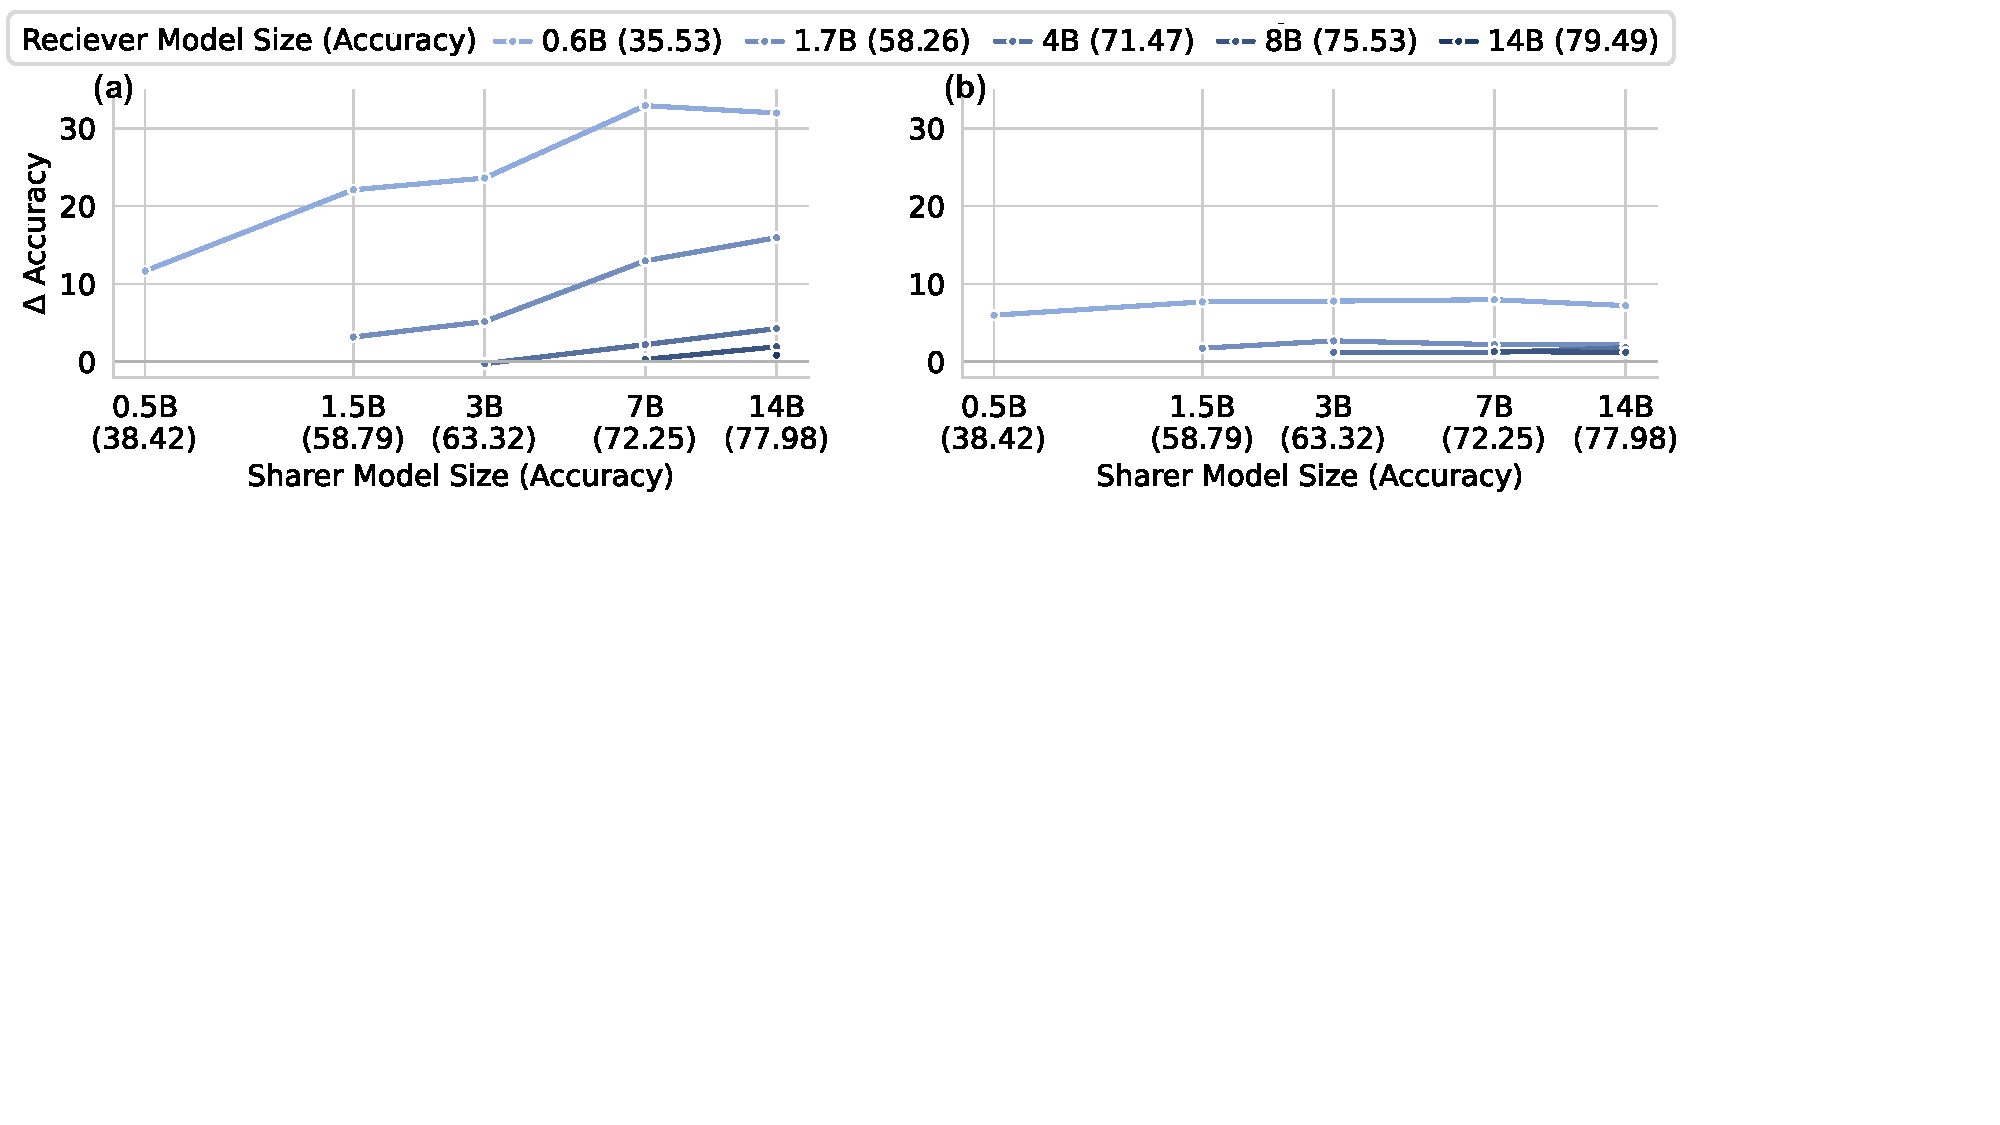
\includegraphics[width=0.95\textwidth]{figure/scaling.pdf}
    \caption{Accuracy improvements ($\Delta$Accuracy) on the MMLU-Redux benchmark. (a) \name communication. (b) T2T communication. The $x$-axis denotes the Sharer model from the Qwen2.5-Instruct series, while the curves correspond to Receiver models from the Qwen3 series. The accuracy improvements of \name generally increase faster than T2T.}
    \label{fig:scaling_behavior}
\end{figure}

\xhdr{Scaling sequence lengths}
We evaluate how \name scales with respect to sequence length on long-context tasks from the LongBenchV1 benchmark. 
All \name fusers are trained and tested on different sets of LongBenchV1.
As shown in Table~\ref{tab:c2c_main}, \name consistently outperforms text-to-text communication across all sequence-length intervals. This demonstrates \name's advantages across input length ranges. 
More detailed setups and results are in Appendices~\ref{sec:appendix/exp/strong2weak} and~\ref{sec:appendix/setup/eval}.
\begin{table}[t]
\centering
\footnotesize
\setlength\tabcolsep{4pt}
\begin{minipage}{0.40\linewidth}
\centering
\setlength\tabcolsep{3pt}
\begin{tabular}{lc|ccc}
\toprule
Length & Receiver & Sharer & T2T & \name \\
\midrule
0-4k & 30.52 & 24.94 & 33.46 & \textbf{37.31} \\
4-8k & 26.03 & 23.18 & 29.70 & \textbf{34.01} \\
8k+   & 25.99 & 16.44 & 25.64 & \textbf{30.72} \\
\bottomrule
\end{tabular}
\caption{Performance scaling with sequence length on LongBenchV1, using Qwen3-0.6B Receiver and Qwen2.5-0.5B Sharer.}
\label{tab:c2c_main}
\end{minipage}
\hfill
\begin{minipage}{0.58\linewidth}
\centering
\setlength\tabcolsep{3pt}
\begin{tabular}{lc|cccc}
\toprule
Setting & \#Param. & OpenBook & ARC-C & MMLU & C-Eval \\
\midrule
Single     & 596M & 45.80 & 47.65 & 36.81 & 35.81 \\
Identical  & 529M & 50.60 & 52.52 & 42.17 & 40.34 \\
\name        & 478M & \textbf{52.60} & \textbf{54.52} & \textbf{42.92} & \textbf{41.77} \\
\bottomrule
\end{tabular}
\caption{Ablation of \name improvement sources. \textit{Single}: fine-tunes Receiver without any Sharer. \textit{Identical}: \name with the same LLM as both Sharer and Receiver. \textit{\name}: use different LLMs as Sharer and Receiver.}
\label{tab:c2c_ablation_train}
\end{minipage}
\end{table}


\xhdr{Scaling model sizes} 
We investigate how \name scales with respect to the Sharer and Receiver model sizes. 
All \name fusers are trained on MMLU's auxiliary train split and evaluated on MMLU-Redux. 
As shown in Figure~\ref{fig:scaling_behavior}, the $x$-axis denotes Sharer size (Qwen2.5-Instruct series), the $y$-axis shows accuracy gains of \name over Receiver-only baselines ($\Delta$ Accuracy), and each curve represents a Receiver from the Qwen3 series. 
We find that the accuracy improvements of \name generally increase faster than T2T.
This trend shows that when the Sharer possesses richer knowledge, \name is able to more effectively transmit useful information to the Receiver. 
Note that the relative gains for larger Receivers are less pronounced due to their stronger baselines and higher overlap with the Sharer’s knowledge.

\xhdr{Different model combinations} 
We test different Sharer-Receiver combinations, including different model families and different task-specific models. 
The result in Table~\ref{tab:c2c_model_combination} shows that \name outperforms text-to-text communication on all five combinations by an average of 8.59\% on MMLU-Redux. This supports that by employing \name, the Receiver model can effectively utilize contextual understanding from different models to enhance performance. 
Notably, when using Qwen2.5-Math as the Sharer, the communication text becomes substantially longer, as analyzed in Appendix~\ref{sec:appendix/result/time}.
To further test the generalizability of \name, we swap the Sharer and Receiver models. The results show that \name robustly brings a 5.05\% increase in accuracy while applying T2T results in a 6.30\% decrease in performance. 

Together, these experiments support the scalability of \name as an effective and efficient new LLM communication paradigm.

\begin{table}[ht]
\centering
\setlength\tabcolsep{3pt} % default value: 6pt
\begin{tabular}{lll|ccccc}
\toprule
Pair Type & Receiver & Sharer    & Metric & Receiver & Sharer & T2T   & \name \\
\midrule
\multirow{6}{*}{Heterogeneous} 
& \multirow{2}{*}{Qwen3-0.6B} & \multirow{2}{*}{Gemma3-1B} & Acc & 35.53 & 31.75 & 41.35 & \textbf{45.90} \\
& & & Time & 0.29 & 0.54  & 1.04  & 0.30 \\
\cmidrule(lr){2-8}
& \multirow{2}{*}{Qwen3-0.6B} & \multirow{2}{*}{Qwen2.5-Math-1.5B}  & Acc & 35.53 & 39.86 & 43.71 & \textbf{46.13} \\
& & & Time & 0.29 & 8.71  & 6.60  & 0.27 \\
\cmidrule(lr){2-8}
& \multirow{2}{*}{Qwen3-0.6B} & \multirow{2}{*}{Qwen2.5-Coder-0.5B} & Acc & 35.53 & 25.09 & 39.74 & \textbf{46.89} \\
& & & Time & 0.29 & 0.26  & 1.59  & 0.27 \\
\midrule
\multirow{4}{*}{Swap} 
& \multirow{2}{*}{Qwen2.5-0.5B} & \multirow{2}{*}{Qwen3-0.6B} & Acc  & 38.42 & 35.53 & 32.12 & \textbf{43.47} \\
& & & Time & 0.34  & 0.29 & 0.98 & 0.21 \\
\cmidrule(lr){2-8}
& \multirow{2}{*}{Qwen3-0.6B} & \multirow{2}{*}{Qwen2.5-0.5B} & Acc & 35.53 & 38.42 & 41.03 & \textbf{46.50} \\
& & & Time & 0.29 & 0.34  & 1.52  & 0.26 \\
\bottomrule
\end{tabular}
\caption{Comparison of Receiver-only, Sharer-only, T2T, and \name across accuracy and time. The pairs are grouped into \textit{heterogeneous} settings (where the Receiver is paired with Sharers of different capabilities) and \textit{swap} settings (where Receiver and Sharer roles are exchanged).}
\label{tab:c2c_model_combination}
\end{table}

\subsection{Ablation Study}
\xhdr{Sources of improvement} 
In Table~\ref{tab:c2c_ablation_train}, we ablate the source of \name performance gain by fixing the Receiver (Qwen3-0.6B) and varying the Sharer. 
\textit{Single} denotes standard full fine-tuning of the Receiver without Sharer. 
\textit{Identical} denotes \name where both Sharer and Receiver are Qwen3-0.6B. 
Our default \name uses Qwen2.5-0.5B as the Sharer. 
Under the same training configuration, \name consistently attains higher accuracy than both \textit{Single} and \textit{Identical}. 
This confirms that \name improvements do not purely come from added trainable capacity or overfitting to the training set. Instead, it points to complementary contextual understanding contributed by the heterogeneous Sharer. \textit{Identical} still outperforms \textit{Single}, indicating that cache-level self-communication can provide useful auxiliary understanding, echoing effects observed in latent reasoning and looped transformers~\citep{saunshi2025loopedTrans, fu2025tah}.

\xhdr{Fuser architecture} In Table~\ref{tab:c2c_ablation} we show the effect of different components in the \name design. Compared with pure projection that discards the Receiver's cache, fusing both models' KV-Caches and retaining the Receiver's via residual connection increases accuracy by 24.18\%. Adding a gate for fused layer selection further increases the average accuracy by 3.07\%.

\begin{table}[tb]
\centering
\begin{tabular}{l|cccccc}
\toprule
Method       & MMLU  & ARC-C & OpenBook & CEval & Average \\
\midrule
Project         & 20.01 & 19.57 & 21.80 & 21.41 & 20.70 \\
    +Fuse      & \textbf{43.36} & 51.65 & 47.60 & 36.91 & 44.88 \\
        +Gate (=\name) & 42.92 & \textbf{54.52} & \textbf{52.60} & \textbf{41.77} & \textbf{47.95} \\
\bottomrule
\end{tabular}
\caption{Ablation of \name fuser components. \textit{Project}: directly replacing the Receiver's KV-Cache with projected Sharer cache. \textit{+Fuse}: fusing both caches and adding the result back to Receiver's via residual. \textit{+Gate}: adding per-layer learnable gating.}
\label{tab:c2c_ablation}
\end{table}

\subsection{Behavior Analysis}

\xhdr{Effective rank analysis} 
We analyze the effective rank of KV-Cache before and after cache-to-cache communication. 
Effective rank~\citep{roy2007effective} is a common measure of the intrinsic dimensionality of model weights or activation values; a higher intrinsic dimension means richer semantic information, as formalized in Appendix~\ref{sec:appendix/setup/effective_rank}.
As Table~\ref{tab:oracle_right} shows, after cache-to-cache fusing, the effective ranks of K and V increased from 388 to 395 and from 532 to 560, respectively. This indicates that \name enriches the semantic space by successfully transforming the Sharer's representations and injecting knowledge into the Receiver model.

\xhdr{Accuracy breakdown}
Our analysis reveals that the source of \name's accuracy gains depends on the relative capacity of the communicating models and varies across task subcategories. Details can be found in Appendix~\ref{sec:appendix/accuracy}. We also find that in some specific cases, C2C may fail as the contextual understanding from the Sharer model is not always accurate and can mislead the Receiver into generating the wrong answer. Representative example is provided in Appendix~\ref{sec:appendix/failure}.

\xhdr{Progressive behavior} We analyze the progressive behavior of \name by gradually increasing the percentage of context KV-Cache being updated by \name (details in Appendix~\ref{sec:appendix/progressive_behavior}).
When the percentage is above 50\%, increasing the percentage continuously yields better performance.

\xhdr{Gate behavior} We analyze the behavior of \name’s learnable gates under different training regimes in Appendix~\ref{sec:appendix/gate}. We can draw the conclusion that general-purpose training favors broad gate activation with fine-grained modulation via weights, whereas task-specific
training favors sparse gate activation with stronger reliance on the selected layers.

